\documentclass[twocolumn]{article}
\usepackage{float}
\usepackage{amsfonts}
\usepackage{amssymb}
\usepackage{amsmath}
\usepackage{cite}
\usepackage{listings}
\usepackage{xcolor}
\usepackage{graphicx}
\usepackage{draftwatermark}
\SetWatermarkText{DRAFT WHITE PAPER}
\SetWatermarkScale{1}

\author{Ryan J. Kung \\ryankung@ieee.org\\Member, IEEE Blockchain Community }
\title{Inferred based Distributed Gaming, Nash Equilibrium}
\begin{document}
\maketitle
% \tableofcontents
\section{Abstract}

Since the introduction of Ethereum on 2014\cite{ethereum}, It brought many DApps and DGames, such as CryptoKitty, Etheremon and Decentraland. Most of them are running into issues addressed to the efficiency of BlockChain implementation, It's too expensive to store data and status in BlockChain like what traditional games does, And it's also can't be worked as a real-time or parity-real-time game during to the delay of transactions. \cite{mrx05}

In this paper, we will studied and discussed how should be a distributed game work on a blockchain based distributed system. First, we discussed distributed nash equilibrium problem, and try to solve the problem with Infered System, finally we will discuss about Zero-knowledge proof as futrue work.

\section{Distributed Nash-Eq}

Like DApps, DGaming is a series of Gaming Behaviors and Strategis which is Decentralized and Distributed. On Lamport's defination on 1978\cite{time-clocks-ordering-events-distributed-system}, A Gaming is Distributed if the message transaction delay is not negligible compared to the time between event in classic gaming behavior. The issues in traditional gaming theory may easily lead us run into trouble if it's distributed, such as nash equilibrium simulation or prisoner's dilemma problem.
On classic Nash Equilibrium, we modeling it with some behaviors table, and proof that for each strategy on game $(S, f)$, and got A strategy profile which is Nash Equilibrium. But on distributed case, the issue is that the event of strategy is not effect immediately, nonnegligible delay of transaction on system may cause N-Eq point out of expectation.



\begin{figure}[H]
  \centering
  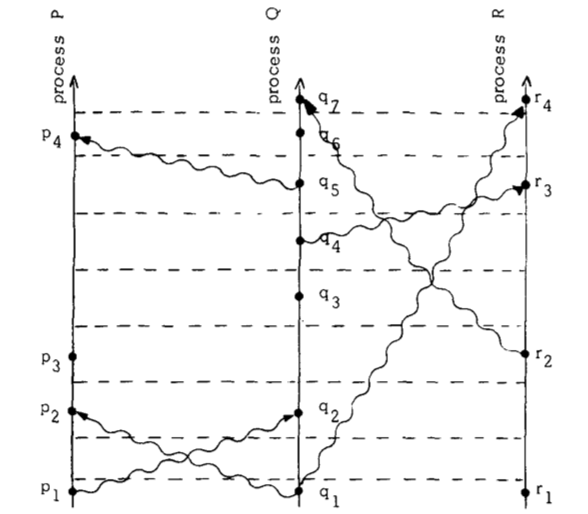
\includegraphics[width=1\linewidth]{img/lamportts.png}
  \caption{Lamport Timestamp}
\end{figure}


In a distributed nash equilibrium case, for example an distributed gaming system build on a simple-paxos based distributed system, actors may try to figure out best response by mining unconfirmed messages as more as they can, which entangled the gaming into a series complicated case, and break perfect information gaming in to imperfect.Actually, Nash equilibrium seeking under communication networks is as tracing increasing attension resently, Some seeking work is about paritially coupled payoff method\cite{8029164}, or Communication Topologies\cite{8093754}. In this paper, we considered distributed Nash equilibrium with a set of player $\mathbb{N} = {1, 2, ..., N}$, under a distributed network which has nonnegligible delay $\mathbb{\delta}$, and Denote $f_i(x)$ as the payoff function of player $i$, where $X = [x_1, x_2, ..., x_n]^T$, $x_i \in S$ is action of player i. And we define a measurement function $m = f(\delta, i)$ which is means how the information is prefect for player $i$.

The distributed equilibrium seeking strategy(DESS) was given by \cite{7888532}:
\begin{gather}
  \dot{x} = k_i \frac {\partial f_i}{\partial x_i}(y_i), i \in \mathbb{N}
\end{gather}

$(\dot{x}^*, 1_N\oplus x^*)$, where $x^*$ presents nash equilibrium. There are some descendent work based on it, but most of them are analytically studied based on certain condition, ignores nonnegligible communication or transaction cost, which is non-ignorable in blockchain and other distributed system. In blockchain case, we can compose measurement function and DESS together, then the strategy can be present as $m(\delta, \dot{x})$. And obviously, there should be existed some relationship between Nash-eq point and $\delta$, such as  $m(\delta_a, \dot{x}) > m(\delta_b, \dot{x}) \iff a > b$. 

\section{Infered perfect information}

Unlike classic distributed system, Blockchain can be seems as a time step function, or a FRP issue which can be abstract as\cite{ElliottHudak97:Fran}, where blockchain Status can be also be abstract as $STMonad$ like MAKERDao\cite{dai}'s work:

\begin{gather}
  time: Status_{time}\\
  at \mathbb{[} time \mathbb{]}t = t
\end{gather}


\section{Pure Functional Solidity}
blalbal

\bibliographystyle{plain}
\bibliography{dgaming}
\end{document}
